\documentclass[conference]{IEEEtran}
\usepackage[backend=biber,dateabbrev=true,style=ieee]{biblatex}

\usepackage{acronym}
\usepackage{algorithm}
\usepackage{algpseudocode} % From 5.1 in http://tug.ctan.org/macros/latex/contrib/algorithmicx/algorithmicx.pdf
\usepackage{amsfonts}
\usepackage{amsmath}
\usepackage{amssymb}
\usepackage{amsthm}
\usepackage{array}
\usepackage{bm}
\usepackage{calc} % For widthof
\usepackage{fontawesome}
\usepackage{hyperref}
\usepackage{pgf}
\usepackage{pgfplots}
\usepackage{pifont}
\usepackage{xparse}

\usepackage[T1]{fontenc}
\bibliography{./bib/bibliography}
% ========================== Basic ==========================
\newcommand{\dyn}[1]{\ensuremath{#1^x}}        % Related to system dynamics
\newcommand{\dst}[1]{\ensuremath{#1^\sigma}}   % Related to system disturbance 

% =========================== Sets ==========================
\renewcommand{\int}{\ensuremath{\mathbb{Z}}}
\newcommand{\real}{\ensuremath{\mathbb{R}}}
\newcommand{\nat}{\ensuremath{\mathbb{N}}}
\newcommand{\cset}{\ensuremath{\mathcal{C}}}

\NewDocumentCommand{\Pre}{ o o m }{%
	\IfNoValueTF{#2}{%
		\IfNoValueTF{#1}{% No #1 or #2
			\ensuremath{\text{Pre}^1\left(#3\right)}
		}{% #1 but no #2
			\ensuremath{\text{Pre}_{#1}^1\left(#3\right)}
		}}{% #1 and #2
			\ensuremath{\text{Pre}^{#2}_{#1}\left(#3\right)}
		}}
\NewDocumentCommand{\PreviewedPre}{ o o m }{%
	\IfNoValueTF{#2}{%
		\IfNoValueTF{#1}{% No #1 or #2
			\ensuremath{\text{Pre}^{\text{\tiny\faEye},1\hspace{-0.1cm}}\left(#3\right)}
		}{% #1 but no #2
			\ensuremath{\text{Pre}_{#1}^{\text{\tiny\faEye},1\hspace{-0.1cm}}\left(#3\right)}
		}}{% #1 and #2
			\ensuremath{\text{Pre}^{\text{\tiny\faEye}, #2\hspace{-0.1cm}}_{#1}\left(#3\right)}
		}}
		
			
% ========================== Ranges =========================
\newcommand{\rgeq}[1]{\ensuremath{_{\geq #1}}}
\newcommand{\rleq}[1]{\ensuremath{_{\leq #1}}}
\newcommand{\rg}[1]{\ensuremath{_{>#1}}}
\newcommand{\rl}[1]{\ensuremath{_{<#1}}}
\newcommand{\rii}[2]{\ensuremath{_{[#1,#2]}}}
\newcommand{\rie}[2]{\ensuremath{_{[#1,#2)}}}
\newcommand{\rei}[2]{\ensuremath{_{(#1,#2]}}}
\newcommand{\ree}[2]{\ensuremath{_{(#1,#2)}}}
\newcommand{\elrii}[2]{\ensuremath{_{\{#1,#2\}}}}

% ===================== Constraint sets =====================
% \_con ----- Produces the constraint set for the indicated quantity. One optional arg adds a substcript.
\NewDocumentCommand{\xcon}{ o o }{%
	\IfNoValueTF{#2}%
	{		
	\IfNoValueTF{#1}%
		{\ensuremath{\mathcal{X}}}%
		{\ensuremath{\mathcal{X}_{#1}}}}
		{\ensuremath{\mathcal{X}{(#1,#2)}}}}
\NewDocumentCommand{\ucon}{ o }{%
	\IfNoValueTF{#1}%
		{\ensuremath{\mathcal{U}}}%
		{\ensuremath{\mathcal{U}_{#1}}}}
\NewDocumentCommand{\tcon}{ o }{%
	\IfNoValueTF{#1}%
		{\ensuremath{\mathcal{T}}}%
		{\ensuremath{\mathcal{T}_{#1}}}}
\NewDocumentCommand{\wcon}{ o o }{%
	\IfNoValueTF{#2}%
		{
		\IfNoValueTF{#1}
			{%
			\ensuremath{\mathcal{W}}%
			}{
			\ensuremath{\mathcal{W}_{#1}}
			}
		}{
		\ensuremath{\mathcal{W}_{#2}^{#1}}
		}}
\NewDocumentCommand{\wconset}{ m }{\ensuremath{\mathfrak{W}^{#1}}}

% ==================== Switching signals ====================
% \ss --------- General switching signal
% \sucset ----- Successor matrix associated with signal #1. Ex. \sucmat{\dyn\ss}
% \sucsetel --- Successor matrix element (#2,#3) associated with signal #1. Ex. \sucset{\dyn\ss}{\dyn\modeidx_i}{\dyn\modeidx_j}

% \mindts ----- Vector of the mode-dependent min-DTs for signal #1. Ex \mindts{\dst\ss}
% \maxdts ----- Vector of the mode-dependent max-DTs for signal #1. Ex \maxdts{\dst\ss}
% \mindt ------ The mode-dependent min-DT for signal #1, mode #2. Ex \mindt{\dst\ss}{\dst\modeidx}
% \maxdt ------ The mode-dependent max-DT for signal #1, mode #2. Ex \maxdt{\dst\ss}{\dst\modeidx}
% \sucsetcon -- Succesoor matrix constraint

% \mindtscon -- Vector of min-dt constraints
% \maxdtscon -- Vector of max-dt constraints
% \mindtcon --- Single min-dt constraint
% \maxdtcon --- Single max-dt constraint
% \ssset     -- Set of switching signals that respects up to three constraint elements

% \sstimer   -- Ss timer. Maps the time and a ss to the number of steps since a switch that new information was gleaned
% \sstimerval - A Value of switching signal timer
% \sstimermax - Maximum value of the switching signal timer in mode #1
% \sspairset -- The set of possible pairs given a mode #1 and timer value #2
% \sscount ---- The number of times the switching signal has changed at some time t

\renewcommand{\ss}{\ensuremath{{\sigma}}}
\newcommand{\sucset}[1]{\ensuremath{\mathcal{S}^{#1}}}
\newcommand{\sucsetrow}[2]{\ensuremath{\sucset{#1}_{#2}}}
\newcommand{\sucsetel}[3]{\ensuremath{{s_{#2,#3}^{#1}}}}

\newcommand{\mindts}[1]{\ensuremath{\underline{\mathcal{D}}^{#1}}}
\newcommand{\maxdts}[1]{\ensuremath{\overline{\mathcal{D}}^{#1}}}
\newcommand{\mindt}[2]{\ensuremath{{\underline{\delta}_{#2}^{#1}}}}
\newcommand{\maxdt}[2]{\ensuremath{{\overline{\delta}_{#2}^{#1}}}}
\newcommand{\sucsetcon}{\ensuremath{{S}}}
\newcommand{\sucsetconrow}[1]{\ensuremath{{S_{#1}}}}

\newcommand{\mindtscon}{\ensuremath{\underline{D}}}
\newcommand{\maxdtscon}{\ensuremath{\overline{D}}}
\newcommand{\mindtcon}[1]{\ensuremath{{\underline{d}_{#1}}}}
\newcommand{\maxdtcon}[1]{\ensuremath{{\overline{d}_{#1}}}}
%\newcommand{\ssset}[3]{\ensuremath{\Sigma(#1,#2,#3)}}
\NewDocumentCommand{\ssset}{ o o o }{%
	\IfNoValueTF{#3}%
		{\IfNoValueTF{#2} %no 3
			{\IfNoValueTF{#1}%no 2, no 3
				{\ensuremath{\Sigma}}
				{\ensuremath{\Sigma(#1)}}
			}
			{\ensuremath{\Sigma(#1,#2)}}%no 3 but 1 and 2
		}
		{\ensuremath{\Sigma(#1,#2,#3)}}}
		
\newcommand{\sstimer}{\ensuremath{{T}}}
\newcommand{\sstimerval}{\ensuremath{\tau}}
%\newcommand{\sstimermax}[1]{\ensuremath{{\overline{\sstimerval}_{#1}}}}
\NewDocumentCommand{\sstimermax}{o m}{%
	\IfNoValueTF{#1}{
		\ensuremath{{\overline{\sstimerval}_{#2}}}
		}{
		\ensuremath{{\overline{\sstimerval}_{#2}^{#1}}}}}
\newcommand{\sspairset}[2]{\ensuremath{{\Lambda((#1,#2))}}}
\newcommand{\sscount}{\ensuremath{{\ss^\#}}}

\newcommand{\switchtimes}[1]{\ensuremath{\tau^{#1}}}
\newcommand{\switchtime}[2]{\ensuremath{{\switchtimes{#1}_{#2}}}}
\newcommand{\lastswitchtime}[1]{\switchtimes{#1}_+}

% ================== System Agents ==================
\newcommand{\agents}{\ensuremath{\mathcal{M}}}
\newcommand{\agent}[1]{\ensuremath{\agents^{#1}}}
\newcommand{\numagents}{\ensuremath{{C_a}}}
\newcommand{\agentidx}{\ensuremath{\alpha}}

% ================== System Modes ==================
% \modes -------- A collection of modes. May optionally specify parent agent.
% \mode --------- A single mode indexed by #1
% \nummodes --- Number of modes 
% \modeidx ------ Index of a single mode \ss(t)=\modeidx

% \nx ------------- The state dimension
% \nu ------------- The input dimension

\NewDocumentCommand{\modes}{o}{%
	\IfNoValueTF{#1}{
		\ensuremath{\mathcal{M}}
		}{
		\ensuremath{\mathcal{M}^{#1}}}}
\NewDocumentCommand{\mode}{o m}{%
	\IfNoValueTF{#1}{
		\ensuremath{\modes{M}_{#2}}
		}{
		\ensuremath{\modes{M}[#1]_{#2}}}}
\NewDocumentCommand{\nummodes}{o}{%
	\IfNoValueTF{#1}{
		\ensuremath{C_m}
		}{
		\ensuremath{{C_m^#1}}}}
\newcommand{\modeidx}{{\ensuremath{\mu}}}

\newcommand{\nx}{\ensuremath{{n_x}}}
\renewcommand{\nu}{\ensuremath{{n_u}}}
\NewDocumentCommand{\futstate}{ o o o o}{%
	\IfNoValueTF{#3}%
		{\ensuremath{x{(#1,#2)}}}
		{\ensuremath{\phi(#1;#2,#3,#4)}}}
\NewDocumentCommand{\useq}{}{\ensuremath{\mathfrak{u}}}
\NewDocumentCommand{\feasuseq}{mmm}{%
	\ensuremath{\mathfrak{U}(#1,#2,#3)}
	}
	
	
% ==================== Safe sets ====================
\newcommand{\safesets}{\ensuremath{\mathcal{S}}}
\newcommand{\safeset}[2]{\ensuremath{\safesets_{(#1,#2)}}}


% ==================== Misc ====================
\newcommand{\narroweq}{\ensuremath{\scalerel[1ex]{=}{\phantom{=}\hspace{-0.17cm}}}}

% ============== Autoref Titles ================
\renewcommand{\equationautorefname}{Equation}
\renewcommand{\sectionautorefname}{Section}
\newcommand{\remarkautorefname}{Remark}
\newcommand{\algorithmautorefname}{Algorithm}
\newacro{mpc}[MPC]{model predictive control}
\newacro{mindt}[min-DT]{minimum dwell time}
\newacro{maxdt}[max-DT]{maximum dwell time}
\newacro{pi}[PI]{positive invariant}
\newacro{ci}[CI]{Control invariant}

\newtheorem{theorem}{\textbf{Theorem}}
\newtheorem{lemma}{\textbf{Lemma}}
\newtheorem{corollary}{\textbf{Corollary}}
\newtheorem{definition}{Definition}
\newtheorem{assumption}{Assumption}
\theoremstyle{remark}
\newtheorem*{remark}{Remark}
\newtheorem{case}{Case}
\newtheorem{problem}{Problem}

\newcommand{\alert}[1]{\textbf{\color{red}{\MakeUppercase{#1}}\color{black}}}

\renewcommand{\theoremautorefname}{Theorem}
\renewcommand{\algorithmautorefname}{Algorithm}
\newcommand{\definitionautorefname}{Def.}
\newcommand{\lemmaautorefname}{Lemma}
\newcommand{\assumptionautorefname}{Assumption}

% For do-while algorithm loops (https://tex.stackexchange.com/questions/115709/do-while-loop-in-pseudo-code)
\algdef{SE}[DOWHILE]{Do}{doWhile}{\algorithmicdo}[1]{\algorithmicwhile\ #1}%
\renewcommand{\algorithmicrequire}{\textbf{Input:}}
\renewcommand{\algorithmicensure}{\textbf{Output:}}
% declaration of the new block
\algblock{ParFor}{EndParFor}
% customising the new block
\algnewcommand\algorithmicparfor{\textbf{parfor}}
\algnewcommand\algorithmicpardo{\textbf{do}}
\algnewcommand\algorithmicendparfor{\textbf{end\ parfor}}
\algrenewtext{ParFor}[1]{\algorithmicparfor\ #1\ \algorithmicpardo}
\algrenewtext{EndParFor}{\algorithmicendparfor}


%\NewDocumentCommand{\edit}{m m}{#2}
\NewDocumentCommand{\edit}{m m}{{\color{red}#1 }{\color{blue}#2}}

\newlength{\myl}
\let\origequation=\equation
\let\origendequation=\endequation
\RenewEnviron{equation}{
  \settowidth{\myl}{$\BODY$}                       % calculate width and save as \myl
  \origequation
  \ifdimcomp{\the\linewidth}{>}{\the\myl}
  {\ensuremath{\BODY}}                             % True
  {\resizebox{\linewidth}{!}{\ensuremath{\BODY}}}  % False
  \origendequation
}

\pgfplotsset{compat=1.17}

\def\BibTeX{{\rm B\kern-.05em{\sc i\kern-.025em b}\kern-.08em T\kern-.1667em\lower.7ex\hbox{E}\kern-.125emX}}
    
\begin{document}
\title{Persistent Feasibility in High Dimension, Externally Switched Systems}

\author{\IEEEauthorblockN{1\textsuperscript{st} Richard A Hall}
\IEEEauthorblockA{\textit{Thomas Lord MEMS Department} \\
\textit{Duke University}\\
Durham, NC, USA \\
0000-0003-3512-6941}
\and
\IEEEauthorblockN{2\textsuperscript{nd} Leila Bridgeman}
\IEEEauthorblockA{\textit{Thomas Lord MEMS Department} \\
\textit{Duke University}\\
Durham, NC, USA \\
0000-0002-9367-7218}
}
\maketitle

\begin{abstract}
Ensuring feasibility in externally switched systems usually requires identifying time-varying, control invariant (CI) sets that ensure state and input constraints can be respected under any possible switching signal. As with traditional, time-invariant CI sets, these time-varying constraints can be very difficult to compute for higher dimensional systems. Furthermore, if multiple switching signals are present, the number of possible permutations of these signal values grows exponentially. Previous works would struggle to account for this growth. Inspired by distributed systems, this work examines a class of high dimensional systems with multiple switching signals. The switching signals are constrained using directed graphs that are much more flexible than dwell time based methods used in much of the previous literature. An iterative algorithm is developed that computes the time-varying CI sets for this class of systems. Critically, this algorithm is parallelized over the number of agents preventing the exponential growth in computation time as agents are added to the system. The scalability of the results results are demonstrated on a randomized numerical example.
\end{abstract}
\section{Introduction}
Hybrid systems are a broad and important class of systems with both discrete and continuous (or discrete approximations of continuous) dynamics. A subclass of these are systems whose discrete dynamics are purely time dependent and unknown to the system. Such discrete, external dynamics can be viewed as an external signal switching the system dynamics at discrete, unforeseen times. 

Many systems experience changes to its dynamics beyond the input of the controller. For example, user input and component failures can both cause the system to suddenly change. If the system is constrained, then special care should be taken to make the system robust to these switches so that constraints are not violated. 

If the system were allowed to be switched arbitrarily, then satisfying the constraints would be restrictive indeed. This would require the controller to always keep the state within a control invariant set common to every modes. If the modes are not extremely similar, this may be a very difficult requirement meet. 

Instead of arbitrary switching, dwell time and successor constraints are often imposed on the switching signal. Minimum dwell time constraints give the system time to recover after a switch and prepare for the next one while maximum dwell time constraints ensure that the system will not dwell in ``poorly'' behaved modes for too long. These constraints can either be generated by the physical implementation and used by the controller or generated by the controller and enforced in the physical implementation.

Dwell time and successor constraints have been used in previous works to create time-varying control invariant sets that are robust to all possible switching signals \alert{cite}. An issue with these previous methods is that they can be very computationally expensive and suffer greatly from the curse of dimensionality. This precludes their use in large systems. 

A further shortcoming of the current literature is that only a single switching signal is considered. It is not difficult to imagine cases where there are multiple sources of switching that are independent from each other. Consider a distributed system where the individual agents are switching according to local switching signals. This independence makes a common switching signal with shared dwell time and successor constraints much more difficult to motivate. Seeking to enumerate the possible states of even just two switching signals and define their dwell time and successor constraints leads quickly back to arbitrary switching but with many more modes.

This work develops an algorithm with applications to both reduce the computational expense of previous algorithms and analyze of systems with multiple sources of switching. The algorithm's most computationally expensive steps are parallelizable, greatly improving its scalability. In the next section, notation and concepts are introduced that will be used throughout the reminder of the paper. Next, the general form of the system is described and the associated challenges are discussed further. Finally, several algorithms are introduced as key contributions of this work and their theoretical properties and implementation are explored. These are then applied to a numerical example that demonstrates the effectiveness of the results. 

Related works includes \cite{Ahandani2020} where the authors examine decentralized systems under MPC with switching communication topologies and coupling in the constraints and inputs. The local agents are assumed LTI while the cross dynamics change according to the switching signal. This leads to an external disturbance applied to each node that is rejected using tube-based, switched MPC.
 \section{Literature Review}
 \subsection{Key contributions of this paper}
 This paper examines systems that
 \begin{enumerate}
 	\item are distributed,
 	\item are coupled through states,
 	\item are uncoupled through constraints,
 	\item have locally switching dynamics,
 	\item have a switching network according to local switches,
 	\item have local, constrained, external switching signals.
 \end{enumerate}
 How does this compare with other papers?

\cite{Ahandani2020} examines decentralized systems under MPC with switching communication topologies and dynamics coupling. The switching is generated from a centralized signal with a minimum dwell time constraint. The local agents are assumed LTI while the cross dynamics change according to the switching signal. This leads to an external disturbance drawn from a switching set applied to each node. This is rejected using tube-based, switched MPC. 

\cite{Monasterios2019} examines systems under MPC that are provided a preview of future disturbances. The preview evolves through disturbed shifting dynamics. The primary results of the paper show that, if the change in disturbance is ``small enough'', the system can maintain feasibility and stability with augmented terminal control elements. It does not, however, consider switching either locally nor remotely. 

\cite{Danielson2019} looks at LTI systems with a single external switching signal that can alter the system's dynamics, constraints, and objectives. It scales poorly, however.

The authors of \cite{Li2020} look at distributed MPC with switching communication topologies. Each agent shares its predicted state trajectory with its neighbors and must stay ``close'' to the trajectory it shared at the last time step. By balancing how much the trajectory may change, the cost of a trajectory change, and terminal constraints, leads to stability. This work does not consider state constraints beyond terminal constraints and does not consider switching in the local dynamics, only the communication network. 
\begin{center}
\renewcommand{\arraystretch}{1.5}
\begin{table}[t]
\begin{tabular}{|m{1cm}|m{6.8cm}|}
\hline
\textbf{Symbol} & \textbf{Description}\\
\hline\hline
$\numagents$ & Number of switching signals/agents\\
\hline
$\agentidxset$ & Set of agent indicies, $\int\rii{1}{\numagents}$\\
\hline
$\nummodes[\agentidx]$ & Number of modes in agent $\agentidx\in\agentidxset$\\
\hline
$\modeidxset[\agentidx]$ & Set of mode indicies in agent $\agentidx$, $\int\rii{1}{\nummodes[\agentidx]}$\\
\hline
\end{tabular}
\end{table}
\end{center}
\section{Preliminaries}
\subsection{Notation}
The set of integers and real numbers are denoted $\int$ and $\real$ respectively. A ranged subset of a space is denoted with $\mathbb{S}\rii{i}{j}=\{s\in\mathbb{S}|i\leq s\leq j\}$. Parenthesis are used in place of brackets to denote strict inequalities. Open bounds are defined using notation such as $\mathbb{S}\rgeq{i}$ where any comparison operator can be substituted for $\geq$. Define the set of integers from $1$ to $k>1$ as $\idxset{k}\triangleq\int\rii{1}{k}$. Use $\PowerSet{\cdot}$ to denote the power set of a finite set.

A directed graph \edit{}{with $\gnumnodes\in\int\rgeq{1}$ nodes} is defined as $\graph\triangleq\{(\gnodeedges{n},\gnodelabel{n})\}_{n\in\idxset{\gnumnodes}}$ where $\gnodeedges{n}\in\PowerSet{\idxset{\gnumnodes}}$ lists the successor nodes of node $n$ and $\gnodelabel{n}=\idxset{\gnumlabels}$ \edit{is the node's label}{is an integer label assigned to node $n$ where $\gnumlabels$ is the max integer label}. A discrete, time varying function, \edit{$f(t)$ mapping to a graph's nodes}{$f:\int\rgeq{0}\rightarrow\idxset{\gnumnodes}$}, is said to respect the graph if $f(t)=n$ implies that $f(t+1)\in\gnodeedges{n}$. The set of all such functions for a specific graph, $\graph$ is denoted $\Sigma(\mathcal{G})\triangleq\{g:\int\rgeq{0}\rightarrow\idxset{\gnumnodes}\ |\ g(\cdot)\text{ respects }\graph\}$. 
\begin{remark}
Note that a function $f(\cdot)\in\Sigma(\graph)$ maps to a node, not the node's label. The active label at time $t$ can be accessed with $\gnodelabel{f(t)}$. 
\end{remark}

\subsection{Switching Signals}
An external switching signal is any discrete function, $\ss(\cdot)$ that is uninfluenced by the system's state and control inputs and causes elements of the plant and/or controller to switch. In this work, the switching signals are constrained using directed graphs \edit{. A directed graph is defined as $\graph\triangleq\{(\gnodeedges{n},\gnodelabel{n})\}_{n\in\idxset{\gnumnodes}}$ where $\gnodeedges{n}\in\PowerSet{\idxset{\gnumnodes}}$ lists the successor nodes of node $n$ and $\gnodelabel{n}=\idxset{\gnumlabels}$ is the node's label. A switching signal that maps to a graph's nodes is said to respect the graph if $\sigma(t)=n$ implies that $\sigma(t+1)\in\gnodeedges{n}$. The set of all such signals for a specific graph, $\graph$ is denoted $\Sigma(\mathcal{G})\triangleq\{\sigma:\int\rgeq{0}\rightarrow\idxset{\gnumnodes}\ |\ \sigma(\cdot)\text{ respects }\graph\}$.}{such that, given the graph $\graph$, $\ss(\cdot)\in\Sigma(\graph)$.} At time $t$, the active node's label indicates the system's mode and is defined as $\ssl(t)\triangleq \gnodelabel{\ss(t)}$. Using directed graphs to constrain the switching signal generalizes dwell time and successor constraints from previous literature, representing a richer set of constraints, as shown in \autoref{fig:graph_ex}.

\begin{figure}[h]
\centering
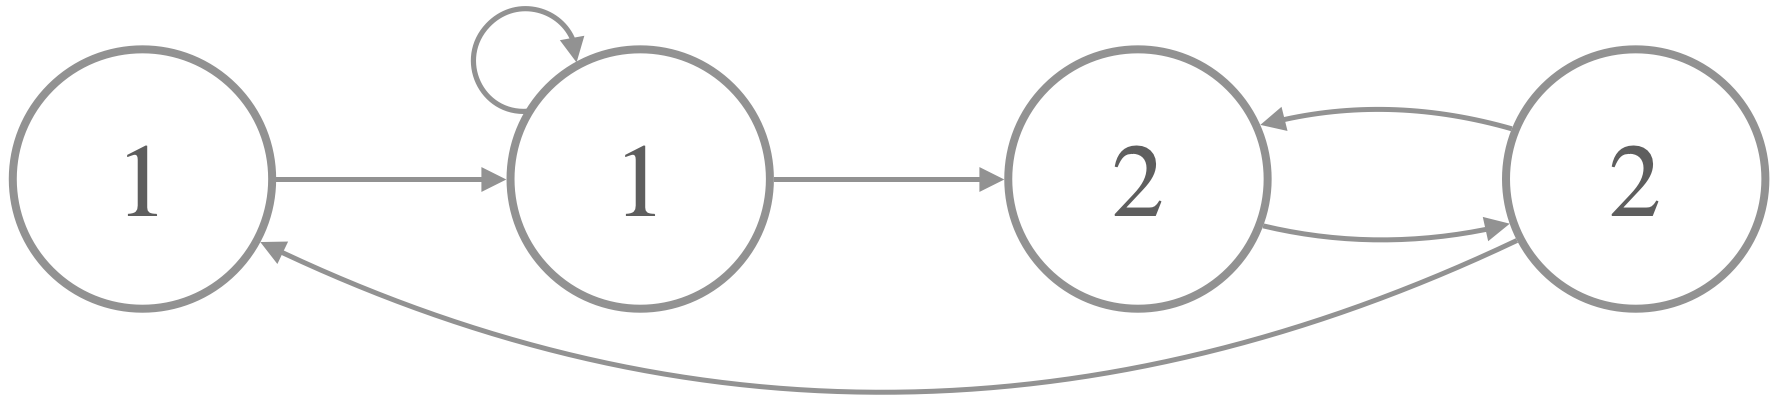
\includegraphics[scale=0.15]{./figures/graph_remark}
\caption{A graph representing a 2-mode system where the first mode has a minimum dwell time of 2 while the second mode can only be left during odd dwell times.}
\label{fig:graph_ex}
\end{figure}

Prior knowledge of the switching signal is not required, but its value at time $t$ is known immediately. Furthermore, its directed graph is known at design time. 
\subsection{General Constrained Switched Systems}
Switched systems are comprised of modes and switching constraints. Each mode contains the dynamics and constraints that the system must respect while the mode is active. A single mode is denoted using the tuple
\begin{equation*}
\mode{\modeidx}\triangleq\{f_\modeidx\in \mathcal{D}^{\nx,\nu,\nw}, \xcon[\modeidx]\subseteq\real^\nx, \ucon[\modeidx]\subseteq\real^\nu, \wcon[\modeidx]\subset\real^\nw\}
\end{equation*}
where $\mathcal{D}^{\nx,\nu,\nw}\triangleq\{f:\real^{\nx\times\nu\times\nw}\rightarrow\real^\nx\}$ defines the set of discrete dynamics,  and $\xcon[\modeidx]$, $\ucon[\modeidx]$, and  $\wcon[\modeidx]$ are the state, input, and disturbance constraints respectively. The full constrained switched system collects the modes and a directed graph to take the form
\begin{equation*}
\modes\triangleq\{\{\mode{\modeidx}\}_{\modeidx\in\idxset{\nummodes}}, \graph\}
\end{equation*}
where the labels of the graph correspond to a mode index, $\gnumlabels=\nummodes$.

\subsection{Set Operations and Control Invariance}
Set operations provide tools to analyze how a mode evolves under allowable inputs. Given a mode, $\mode{\modeidx}$, the following important set operation is introduced. 
%\begin{definition}[Robust Preset]\label{def:robust_preset}
%The $k$-step, robust preset of a set $\mathcal{S}$ under the constrained dynamics $\mode{\modeidx}$ is given by
%\begin{align}
%\Pre[\modeidx][0]{\mathcal{S}}&\triangleq\mathcal{S},\\
%\Pre[\modeidx][k]{\mathcal{S}}&\triangleq\{x\in\xcon[\modeidx]\ |\ \exists u\in\ucon[\modeidx]\text{ s.t. }\forall w\in\wcon[\modeidx],\nonumber\\ &\qquad f_\modeidx(x,u,w)\in\Pre[\modeidx][k-1]{\mathcal{S}}\}.
%\end{align}
%\end{definition}
\begin{definition}[Previewed Robust Preset]\label{def:prev_robust_preset}
The $k$-step, previewed robust preset of a set $\mathcal{S}$ under the constrained dynamics $\mode{\modeidx}$ is given by
\begin{align}
\PreviewedPre[\modeidx][0]{\mathcal{S}}&\triangleq\mathcal{S},\\
\PreviewedPre[\modeidx][k]{\mathcal{S}}&\triangleq\{x\in\xcon[\modeidx]|\forall w\in\wcon[\modeidx],\exists u\in\ucon[\modeidx]\text{ s.t. }\nonumber\\
&\hspace{1.85cm} f_\modeidx(x,u,w)\in\PreviewedPre[\modeidx][k-1]{\mathcal{S}}\}.
\end{align}
\end{definition}
Comparing this to the more common robust preset operator, the previewed robust preset is allowed to select the input based on a known disturbance. The previewed robust preset is used when the system is allowed a preview of the current disturbance. This preview can expand the size of the preset because the selected input need not handle every possible disturbance. 

For linear systems where $f_\modeidx(x,u,w) = A_\modeidx x + B_\modeidx u + E_\modeidx w$, previewed robust presets can be found using basic set operations such as the Minkowski sum and difference as shown below and adapted from \cite{Borrelli2017}.
\begin{align*}
\PreviewedPre[\modeidx][1]{\mathcal{S}} &= \left(\left(\left(\mathcal{S}\oplus\left(-B_\modeidx\circ\ucon[\modeidx]\right)\right)\ominus E_\modeidx\circ\wcon[\modeidx]\right)\circ A_\modeidx\right)\ \cap\ \xcon[\modeidx].
\end{align*}

Preset operations are critical in the calculation of invariant sets commonly used in feasibility analysis. An invariant set is defined as follows.
\begin{definition}[\Ac{ci} sets \cite{Dorea1999}]\label{def:ci_set}
A set, $\mathcal{S}\subseteq\xcon[\modeidx]$ is CI under mode $\mode{\modeidx}$ if for all $x\in\mathcal{S}$, there exists a $u\in\ucon[\modeidx]$ such that \edit{$f_\modeidx(x,u,w)\in\mathcal{S}$.}{$f_\modeidx(x,u,0)\in\mathcal{S}$. Likewise, a set $\mathcal{S}\subseteq\xcon[\modeidx]$ is a previewed robust CI (PR-CI) set if, for all $x\in\mathcal{S}$ and $w\in\mathcal{W}_\modeidx$, there exists a $u\in\ucon[\modeidx]$ such that $f_\modeidx(x,u,w)\in\mathcal{S}$.} Equivalently, $\mathcal{S}$ is CI\edit{}{ (PR-CI)} iff $\mathcal{S}\subseteq\Pre[\modeidx][1]{\mathcal{S}}$\edit{.}{ where the preset operator is nominal (previewed robust).}
\end{definition}
\edit{ This definition holds regardless of if the preset operator is nominal, robust, or previewed robust.}{}

A final tool used in this paper is the convex hull of a set defined as follows.
\begin{definition}[Convex Hull]
Given a set $\mathcal{S}\subseteq\real^n$, the convex hull is defined as 
\begin{align*}
&\Call{ConHull}{\mathcal{S}}\triangleq\\&\{x\in\real^n\ |\ \exists\ a,b\in\mathcal{S},\ \gamma\in\real\rii{0}{1}\ \text{s.t.}\ x=\gamma a + (1-\gamma)b\}.
\end{align*}
\end{definition}
\subsection{Feasibility Analysis}
In constrained systems, it is extremely important that the controller can satisfy the state constraints using only feasible inputs. If a feasible input exists that results in a feasible state, the system is feasible. If feasibility at the current time implies feasibility at all future times, then the system is persistently feasible.

In centralized, unswitched systems, persistent feasibility can be established by constraining the system to be within a \ac{ci} set, $\mathcal{C}\subseteq\mathcal{X}$ \cite{Blanchini1999}. Relying on constant, control invariant sets becomes difficult in externally switched systems, however. The \ac{ci} set must be common to all system modes or else persistent feasibility is lost. This concern can be addressed using time varying, control invariant sets that take advantage of constraints on the switching signal. For example, in \cite{Danielson2019,Santis2004,Lavaei2021}, time varying, control invariant sets were developed that force the system to move during the dwell time between switches to a region from which a switch to any successor mode will preserve persistent feasibility. By bounding the dwell time below, the system had additional time to reach these safe regions, thereby loosening the state constraints.

The approaches used in the previous literature can be described using safe-set collections. These are collections of sets, indexed by the switching signal, that serve as time-varying state constraints of the system. To establish persistent feasibility, every safe-set must be within the 1-step preset of all possible successor safe-sets. This is presented formally in the following definition.
\begin{definition}[Safe-set collection]
Let the external switching signal, $\ss\in\Sigma(\graph)$ govern the system $\modes\triangleq\{\{\mode{\modeidx}\}_{\modeidx\in\idxset{\nummodes}}, \graph\}$. A collection of sets indexed by the nodes of $\graph$, $\mathcal{S}=\{\mathcal{S}_{i}\}_{i\in\idxset{\gnumnodes}}$ is a safe-set collection if
$$\mathcal{S}_{i}\subseteq\Pre[\gnodelabel{j}][1]{\mathcal{S}_{j}}\ \forall\ i\in\idxset{\gnumnodes},\ j\in \gnodeedges{i}$$
\end{definition}
Safe set collections create target sets for the system to move into at each time step. The preset condition ensures that, no matter how $\ss$ evolves, the system will always be able to find a feasible input to move into the current target set.

%\begin{figure*}[t]
%\centering
%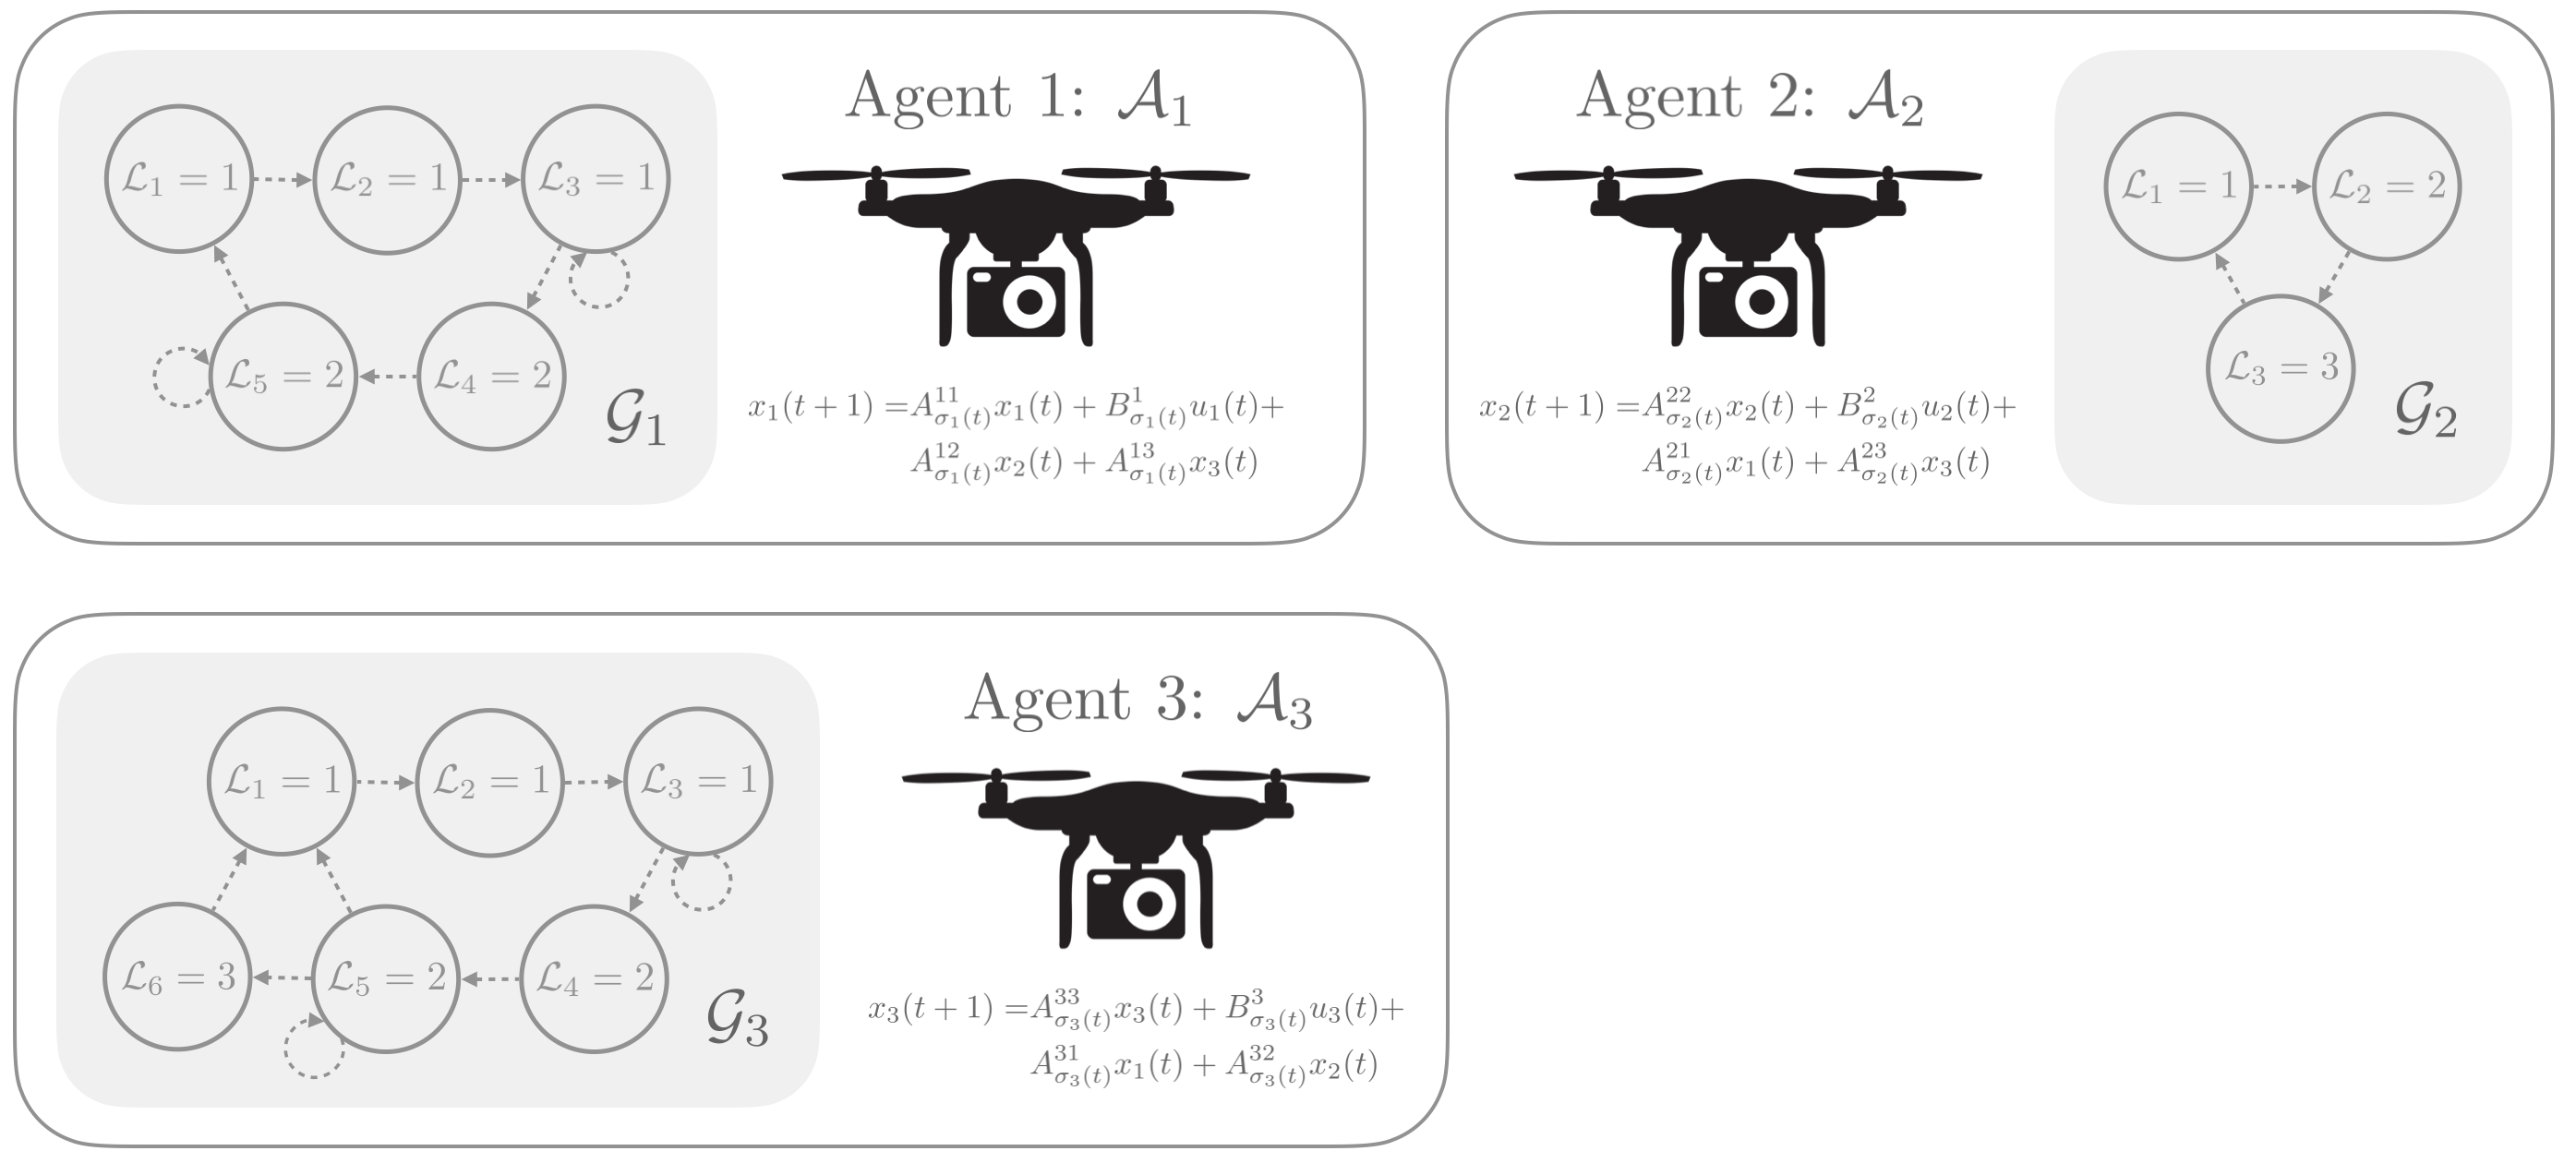
\includegraphics[width=\textwidth]{./figures/sample_system}
%\end{figure*}

\section{System Description}
Consider a collection of $\numagents\in\int\rgeq{1}$ external switching signals each respecting their own directed graph, $\ss_\agentidx(t)\in\Sigma(\graph_\agentidx)\ \agentidx\in\idxset{\numagents}$. Then the dynamics of the system being studied take the following form
\begin{align}
A(t)&=\begin{bmatrix}
A^{11}_{\ss_1(t)}&A^{12}_{\ss_1(t)}&\cdots&A^{1\numagents}_{\ss_1(t)},\\
A^{21}_{\ss_2(t)}&A^{22}_{\ss_2(t)}&\cdots&A^{2\numagents}_{\ss_2(t)},\\
\vdots&\vdots & \ddots & \vdots\\
A^{\numagents 1}_{\ss_\numagents(t)} & A^{\numagents 2}_{\ss_\numagents(t)} &\cdots & A^{\numagents \numagents}_{\ss_\numagents(t)} 
\end{bmatrix},\\
B(t)&=\begin{bmatrix}
B^{1}_{\ss_1(t)}&0&\cdots&0,\\
0&B^{2}_{\ss_2(t)}&\cdots&0,\\
\vdots&\vdots & \ddots & \vdots\\
0 & 0 &\cdots & B^{\numagents}_{\ss_\numagents(t)} 
\end{bmatrix}.
\end{align}
This structure is motivated by distributed systems with coupling in the system's states. Note how each block-row is governed by a single switching signal. This makes intuitive sense because local switching signals are more likely to effect how neighboring states impact the local agent rather then how local states will effect neighboring agents.

Our objective is to design safe-set collections for systems with the above structure. Recall that every element in a safe-set collection must be within the one-step preset of the elements indexed by the possible states of the switching signal after a single time step. The structure of the system under consideration makes this an especially challenging prospect for two reasons. First, the number of successor safe-sets grows exponentially when there are two or more independent switching signals. Second, systems that take this form would likely be in a relatively high dimension making set-operations exponentially more expensive. These two challenges suggest that previous, set-based techniques will struggle due to poor scaling in both the state dimension and the number of modes. These concerns will be addressed by splitting the system into block-rows and looking for safe-set collections for each separately. Once found, the collections can be merged into a large collection with all possible switching signal states represented.

\subsection{Block-row Dynamics}
Looking only at the block row indexed by $\agentidx$, the dynamics can be rewritten as 
\begin{align}\label{eq:block-row-dyn}
x_\agentidx(t+1)&=A^{\agentidx\agentidx}_{\ss_\agentidx(t)}x_\agentidx(t)+B^\agentidx_{\ss_\agentidx(t)}u_\agentidx(t)\nonumber\\&\quad+\sum_{\tilde\agentidx\in\idxset{\numagents}\setminus \agentidx}A^{\agentidx\tilde\agentidx}_{\ss_\agentidx(t)}x_{\tilde\agentidx}(t)\\
=A^{\agentidx}_{\ss_\agentidx(t)}&x_\agentidx(t)+B^\agentidx_{\ss_\agentidx(t)}u_\agentidx(t)+E^\agentidx_{\ss_\agentidx(t)}\left[x_{\tilde\agentidx}(t)\right]_{\tilde\agentidx\in\idxset{\numagents}\setminus \agentidx}.
\end{align}
These dynamics and constraints are collected into the following tuple defining agent $\agentidx$,
$$\agent{\agentidx}\triangleq\{\{A^{\agentidx}_{\modeidx},B^\agentidx_{\modeidx},E^\agentidx_{\modeidx},\xcon[\modeidx]^\agentidx,\ucon[\modeidx]^\agentidx\}_{\modeidx=1}^{\nummodes[\agentidx]},\graph^\agentidx\}.$$

This system only has a single switching signal explicitly appearing, $\ss_\agentidx(t)$, and resembles a locally switched system with additive disturbances. The safe-set collection for this system Previous, robust switched techniques, such as those developed in \cite{Lavaei2021}, may seem like possible solutions. However, these previous techniques rely on bounded additive disturbances and the bounds on $\left[x_{\tilde\agentidx}(t)\right]_{\tilde\agentidx\in\idxset{\numagents}\setminus \agentidx}$ are not obvious. The full state constraints, $x_{\tilde{\agentidx}}\in\xcon[\tilde{\agentidx}]$, could be used but this would lead to conservative results. Alternatively, the current safe-set containing $x_{\tilde{\agentidx}}$ could be used. This however, returns the system to the centralized problem with its associated drawbacks. Furthermore, if \autoref{eq:block-row-dyn} represents a distributed system, this level of communication may be undesirable. Balancing these considerations, this work bounds the neighboring states within the convex hull of the union of the neighbor's safe-set collection. This only requires acquiring a single set and only relies on the state of the local switching signal. 

The reader may have noticed that a circular dependency arose in the previous discussion -- the safe-set collection for agent $\agentidx$ depends on the safe-set collection for agent ${\tilde{\agentidx}}$ which depends on the safe-set collection for agent $\agentidx$. This problematic cycle is addressed in the algorithm development covered in the following section. 
\section{Algorithm Design}
Before addressing the circular dependency mentioned in the previous section, an algorithm to find the safe-sets of a single agent is developed. To avoid the circular dependency, it is assumed that the other agents have fixed safe-sets. Then the disturbance caused by the neighboring agents can be bound with
\begin{equation}
\wcon[\agentidx][\modeidx]=\prod_{\tilde{\agentidx}\in\idxset{\numagents}}\Call{ConHull}{\cup\mathcal{S}^{\tilde{\agentidx}}}.
\end{equation}
With these sets, \autoref{alg:node_safe_sets} is introduced to compute the maximal safe-set collections for this mode. 
\begin{algorithm}[t]
\caption{Nodal safe-sets with previewed disturbances}\label{alg:node_safe_sets}
\begin{algorithmic}[1]
\Procedure {AgentSafeSets}{$\agent{\agentidx}$}
\State $k\gets0$
\State $\Omega_{n}^k\gets\xcon[\gnodelabel{n}]$ for all $n\in\idxset{\gnumnodes[\agentidx]}$.
\Repeat 
	\State $k\gets k+1$
	\For{$n\in\idxset{\gnumnodes[\agentidx]}$}
		\State $\Omega_{n}^k\gets\Omega_{n}^{k-1}$
		\For{$\tilde{n}\in\gnodeedges[\agentidx]{n}$}
				\State $\Omega_{n}^k\gets\Omega_{n}^k\cap\PreviewedPre[\gnodelabel{\tilde{n}}][1]{\Omega_{\tilde{n}}^{k-1}}$
			\EndFor
	\EndFor
\Until{$\Omega_{n}^k=\Omega_{n}^{k-1}\ \forall\ n\in\idxset{\gnumnodes[\agentidx]}$.}
\State $\safeset{}^\agentidx\gets\{\Omega_{n}^k\}_{n\in\idxset{\gnumnodes[\agentidx]}}$.\;
\EndProcedure
\end{algorithmic}
\end{algorithm}

\begin{remark}
An important distinction between this algorithm and previous algorithms focused on robust control is the use of the previewed robust preset operator. This operator is used in place of the more common robust preset operator to increase the size of the resulting safe-sets. Its use only assumes that each block-row is aware to the states of other block-rows prior to selecting a control action. This is a minor assumption that requires little communication overhead.
\end{remark}
\autoref{alg:node_safe_sets} is supported with the following lemmas. 
\begin{lemma}\label{lemma:maximal_proof}
Given any agent, $\agent{\agentidx}$, $\Call{AgentSafeSets}{\agent{\agentidx}}$ returns the maximal safe-set collection.
\end{lemma}
\begin{proof}
Follows the logic of \cite[Theorem 2]{Danielson2019} but with previewed preset operations.
\end{proof}
\begin{lemma}
Let $\agent{\tilde\agentidx}$ and $\agent{\hat\agentidx}$ be two switched systems that are equivalent except for their disturbance bounds which satisfy $E_{\modeidx}^{\agentidx}\circ\wconset{\tilde\agentidx}_\modeidx\subseteq E_{\modeidx}^{\agentidx}\circ\wconset{\hat\agentidx}_\modeidx$ for each mode where $E_{\modeidx}^{\agentidx}=E_{\modeidx}^{\tilde\agentidx}=E_{\modeidx}^{\hat\agentidx}$. Then the relationship
$$\Call{AgentSafeSets}{\agent{\tilde\agentidx}}\supseteq\Call{AgentSafeSets}{\agent{\hat\agentidx}}$$
also holds element-wise. 
\end{lemma}
\begin{proof}
This is proved by contradiction. Let $n\in\idxset{\gnumnodes[\tilde\agentidx]}$ be some node for which $\exists\ x\not\in\mathcal{S}_n^{\tilde{\agentidx}}\ \land\ x\in\mathcal{S}_n^{\hat{\agentidx}}$. Since \autoref{alg:node_safe_sets} is subtractive, there exists some minimal $k\in\int\rgeq{0}$ such that $\exists\ x\not\in\tilde\Omega^k_{n}\ \land\ x\in\hat\Omega^k_{n}$. This implies that there exists a node neighboring $n$, $m\in\gnodeedges[\agentidx]{n}$ with label $\ell_m$, such that there exists an $x$ that violates the preset condition found on line 9 of the algorithm for  $\agent{\tilde\agentidx}$ while respecting it for  $\agent{\hat\agentidx}$.  Using \autoref{def:prev_robust_preset}, this can be stated as $\exists\ x\ \st${\small
\begin{align*}
\exists w\in\wcon[{\ell_m}]^{\tilde{\agentidx}}\ \st\ \forall\ u\in\ucon[{\ell_m}]^\agentidx,\ A_{\ell_m}^\agentidx x+B_{\ell_m}^\agentidx u + E_{\ell_m}^\agentidx w \not\in \tilde\Omega^{k-1}_{{\ell_m}}
\end{align*}}
and{\small
\begin{align*}
\forall w\in\wcon[{\ell_m}]^{\hat{\agentidx}}\ \st\ \exists\ u\in\ucon[{\ell_m}]^\agentidx,\ A_{\ell_m}^\agentidx x+B_{\ell_m}^\agentidx u + E_{\ell_m}^\agentidx w \in \hat\Omega^{k-1}_{{\ell_m}}
\end{align*}}
where the decorations on the $\agentidx$ have been dropped on equivalent values between the two systems. By the relationship given in the lemma body, the second statement above would hold even if $\wcon[{\ell_m}]^{\hat{\agentidx}}$ were replaced with $\wcon[{\ell_m}]^{\tilde{\agentidx}}$. Let $z$ be the corresponding point for which $\exists w\in\wcon[{\ell_m}]^{\tilde{\agentidx}},\ u\in\ucon[{\ell_m}]^\agentidx$ such that $z\not\in\tilde\Omega^{k-1}_{m}\ \land\ z\in\hat\Omega^{k-1}_{m}$. This is equivalent to the starting condition only at a new state and node and with a decremented index. The above logic can be iterated until $k=0$ and the contradiction $\xcon[\ell_n] = \tilde\Omega^0_{n}\subset\hat{\Omega}^0_{n}=\xcon[\ell_n]$ is arrived at, concluding the proof. 
\end{proof}

\autoref{alg:node_safe_sets} is an important tool but requires that the safe-sets of the other block-rows are already known. As mentioned in the previous section, there is a circular dependency where the neighboring safe-sets depend on the local safe-sets which, using \autoref{alg:node_safe_sets}, depends on the neighboring safe-sets. This circular dependency is addressed in \autoref{alg:safe_sets}. Starting from an initial, trivial guess for feasible, safe-set collections, the algorithm first generates safe-sets that are too large and infeasible and then safe-sets that are small but feasible. This process is repeated until a convergence criteria is met. Critically, the algorithm can be parallelized along the different block-rows. As block-rows are added, the computational complexity grows at a near linear rate as opposed to the exponential rate of the centralized case. Furthermore, as shown in the following lemma the algorithm produces a feasible collection of safe-sets after each complete iteration. This allows the user to terminate after any complete iteration and produce valid results. 
\begin{algorithm}[t]
\caption{Distributed safe-set collection for system in \autoref{eq:agent_notation}}\label{alg:safe_sets}
\begin{algorithmic}[1]
\Procedure {SystemSafeSets}{$\agents$}
\State $\Omega^0\gets\{\{\underline{0}\}_{n\in\idxset{\gnumnodes[\agentidx]}}\}_{\agentidx\in\mathcal{I}_\agentidx}$
\State $\Phi^0\gets\{\underline{0}\}_{\agentidx\in\mathcal{I}_\agentidx}$
\State $k\gets0$
\Repeat
	\ParFor{$\agentidx\in\mathcal{I}_\agentidx$}
		\State $\wcon[\modeidx]^\agentidx\gets\prod_{\tilde{\agentidx}\in\idxset{\numagents}}\Phi^{k}_{(\tilde\agentidx)}$ for all $\modeidx\in\idxset{\nummodes[\agentidx]}$
	\EndParFor
	\ParFor{$\agentidx\in\mathcal{I}_\agentidx$}
		\State $\Omega^{k+0.5}_{(\agentidx)}\gets\Call{AgentSafeSets}{\modes[\agentidx]}$
		\State $\Phi^{k+0.5}_{(\agentidx)}\gets\Call{ConHull}{\bigcup\Omega^{k+0.5}_{(\agentidx)}}$
	\EndParFor
	\ParFor{$\agentidx\in\mathcal{I}_\agentidx$}
		\State $\wcon[\modeidx]^\agentidx\gets\prod_{\tilde{\agentidx}\in\idxset{\numagents}}\Phi^{k+0.5}_{(\tilde\agentidx)}$ for all $\modeidx\in\idxset{\nummodes[\agentidx]}$
	\EndParFor
	\ParFor{$\agentidx\in\mathcal{I}_\agentidx$}
		\State $\Omega^{k+1}_{(\agentidx)}\gets\Call{AgentSafeSets}{\modes[\agentidx]}$
		\State $\Phi^{k+1}_{(\agentidx)}\gets\Call{ConHull}{\bigcup\Omega^{k+1}_{(\agentidx)}}$
	\EndParFor
	\State $k\gets k+1$
\Until{$\Omega_{(\agentidx)}^k=\Omega_{(\agentidx)}^{k-1}\ \forall\ \agentidx\in\mathcal{I}_\agentidx$}

\State $\safesets\gets\Omega^k$
\EndProcedure
\end{algorithmic}
\end{algorithm}

\begin{lemma}
The algorithm $\Call{SystemSafeSets}{\agents}$ produces a valid safe-set collection for every $k\in\int\rgeq{0}$. 
\end{lemma}
\begin{proof}
This holds trivially for $\Omega^0$. The following induction steps complete the proof.
\begin{enumerate}
	\item Assume $\Omega^k$ is valid under the disturbance constraints $\Phi^k$.
	\item By Lemma 1, $\Omega^k\subseteq\Omega^{k+0.5}$.
	\item By Lemma 2, $\Phi^k\subseteq\Phi^{k+0.5}$ implies that $\Omega^{k+1}\subseteq\Omega^{k+0.5}$.
	\item Since $\Omega^{k+1}$ is valid for $\Phi^{k+0.5}$, it will also be valid for $\Phi^{k+1}$ since $\Phi^{k+1}\subseteq\Phi^{k+0.5}$.
\end{enumerate}
\end{proof}
\section{Numerical Example}
\begin{figure}
	\centering
	\begin{subfigure}[c]{0.475\columnwidth}%
		\centering
		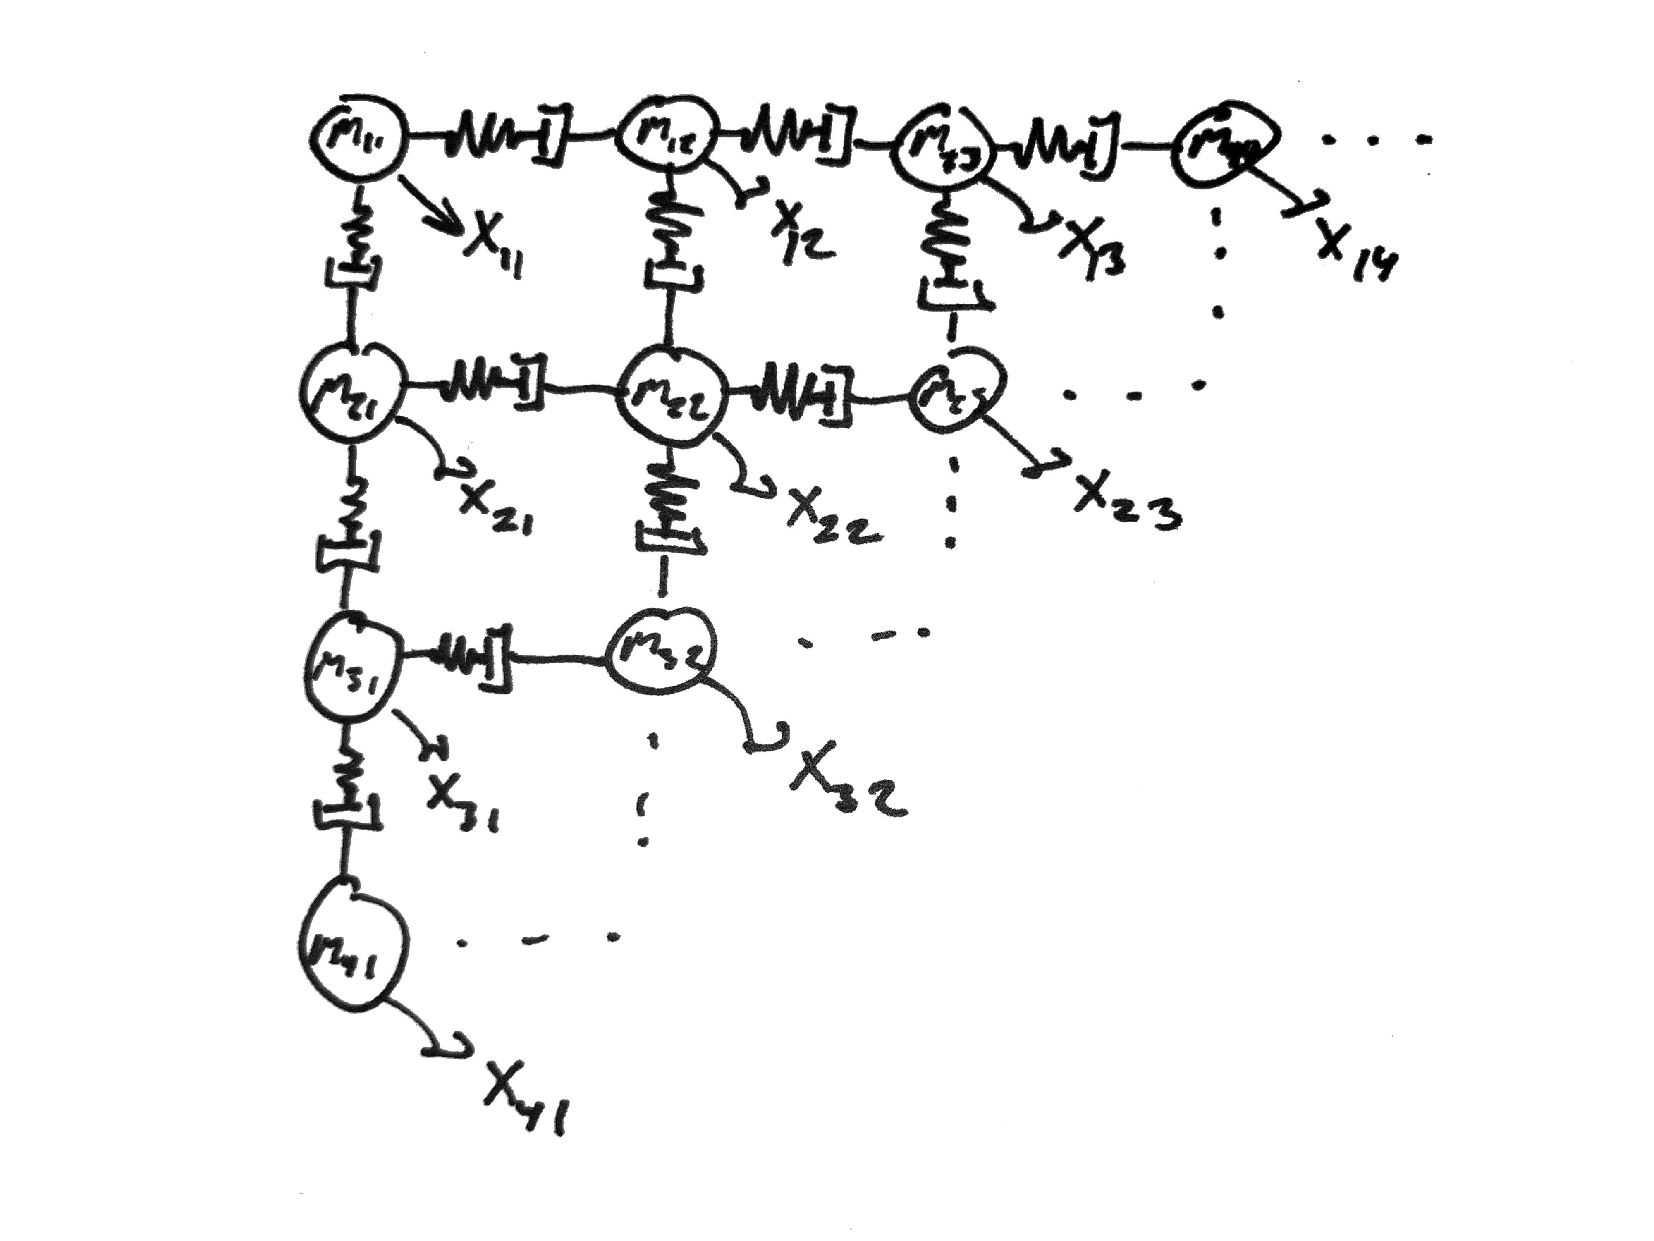
\includegraphics[width=\textwidth]{./figures/num_ex_sys}%
		\caption{Array of linked spring-mass-damper systems. The mass of each object can switch independently according to a directed graph.}%
		\label{fig:num_ex_sys}%
	\end{subfigure}%
	\hfill
	\begin{subfigure}[c]{0.475\columnwidth}%
		\centering
		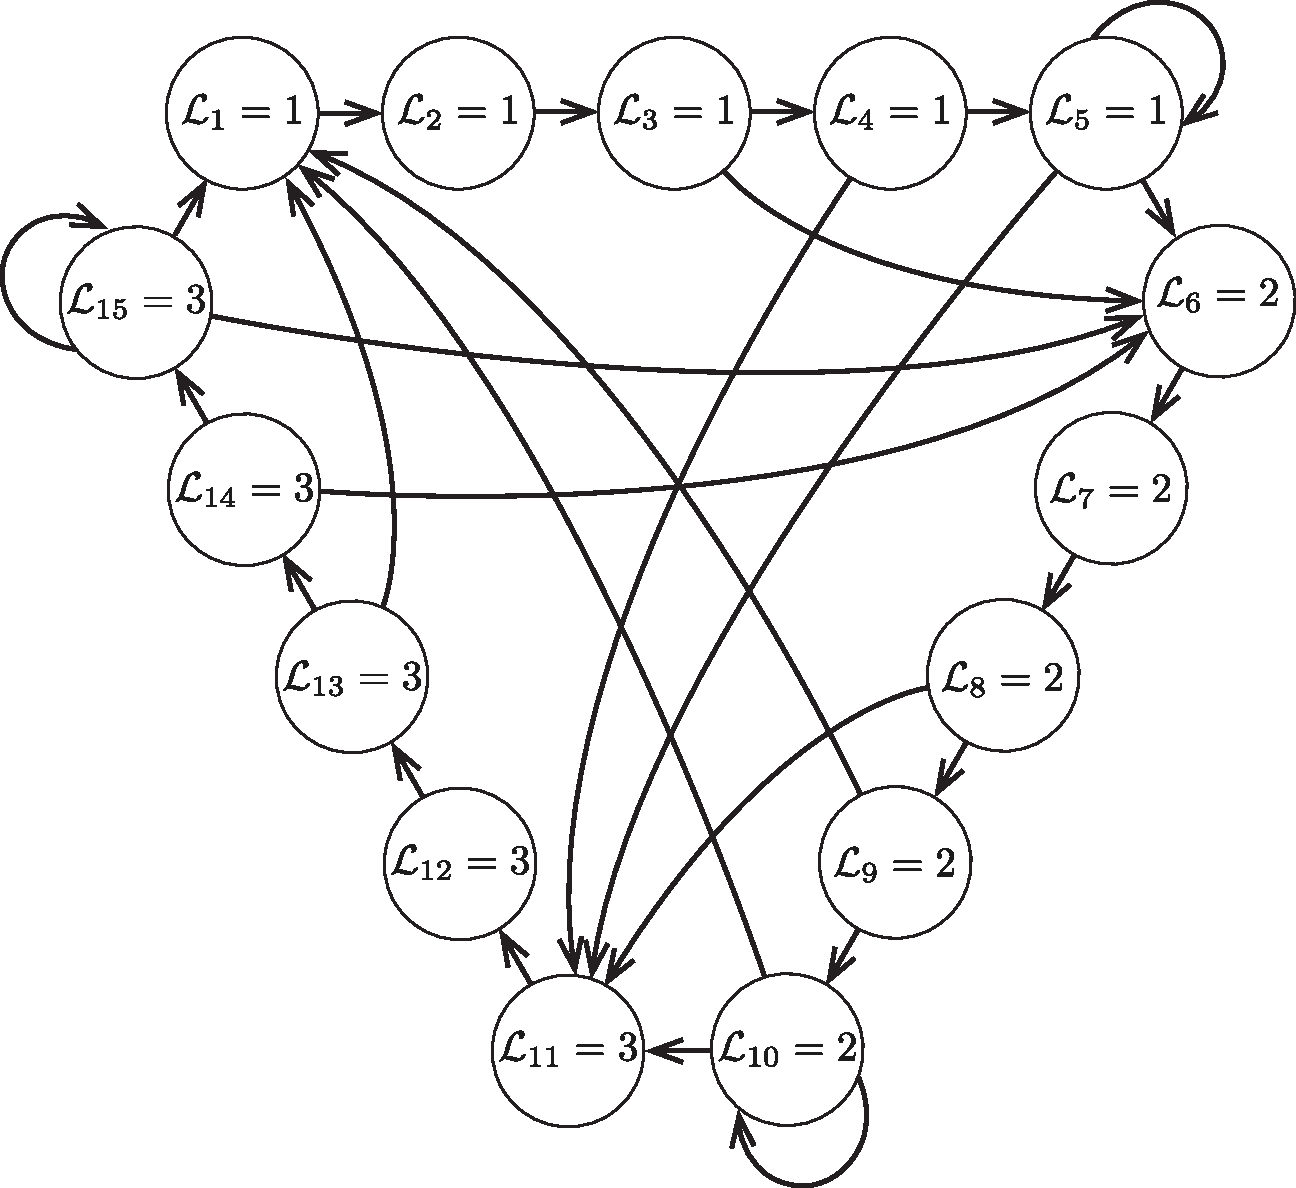
\includegraphics[width=0.8\textwidth]{./figures/num_ex_graph}%
		\caption{Directed graph controlling the switches of the numerical example. Note that the switching constraints cannot be encoded with minimum and maximum dwell times and demonstrate the flexibility of the proposed approach.}%
		\label{fig:num_ex_graph}%
	\end{subfigure}%
	\caption{Description of the system used in the example.}%
\end{figure}

\begin{figure}[t]
\centering
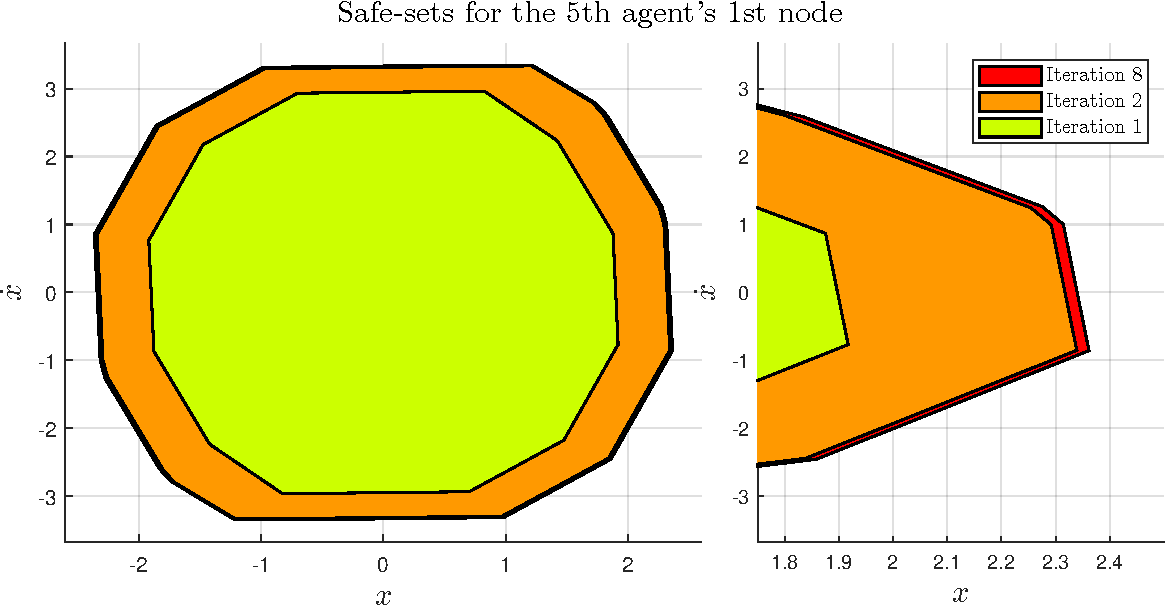
\includegraphics[width=\columnwidth]{./figures/num_ex_results}
\caption{Evolution of the safe-set for a single node of a single agent in the spring-mass-damper array. Though each safe-set shown is feasible, they monotonically increase to convergence with the number of iterations.}
\label{fig:num_ex_results}
\end{figure}

The results of this work are demonstrated in an array of independently controlled agents coupled with springs and dampers as shown in \autoref{fig:num_ex_sys}. The objects move in the dimension denoted by $x_{i,j}$. The mass of each agent can switch between one of three values according to the directed graph shown in \autoref{fig:num_ex_graph}. \edit{}{The linearized dynamics of the top left system is given here as an illustration 
\begin{align*}
m_{11}(\ss_{11}(t))\ddot{x}_{11}(t) = &k_{11|12}(x_{12}(t)-x_{11}(t))\\
+&k_{11|21}(x_{21}(t)-x_{11}(t))\\
+&b_{11|12}(\dot x_{21}(t)-\dot x_{11}(t))\\
+&b_{11|21}(\dot x_{21}(t)-\dot x_{11}(t)) + u_{11}(t)
\end{align*}
 where the spring and dampener coefficients have been scaled to account for the angle at which they apply their force. These dynamics where discretized for each agent at a sampling time of $0.3$ seconds.} For a system comprised of an $r\times c$ array of linked spring-mass-damper systems, the full state space will be in $\real^{2rc}$. Even for small, $2\times 2$ systems, the resulting 8D system is \edit{currently}{} too large for previous set based methods on a conventional PC. However, using the results of this work to parallelize the algorithm, only set operations in $\real^2$ are required. Assuming each agent has it's own independent processing, the computational complexity will grow at a sub-exponential rate with the number of agents. Running \autoref{alg:safe_sets} on the spring-mass-damper grid with randomized masses and spring/damper coefficients resulted in the safe-set evolution shown in \autoref{fig:num_ex_results} for mode 1 of node 1. The numerical example implementation has been archived for the interested reader \cite{PaperSoftware}. 
\section{Conclusion}
In the previous literature ensuring persistent feasibility in externally switched systems, the curse of dimensionality has prevented the study of large scale systems. Furthermore, this computational inefficiency has limited these previous methods' application to systems with multiple switching signals. This work addresses both of these difficulties in systems representing distributed systems coupled through their states. A graph based constraint scheme was described to constrain each agent's switching signal that provides much greater flexibility than previous dwell time constraints. Iterative algorithms where then developed that efficiently computed time-varying state constraints that, when respected, ensure feasibility under all permutations of the switching signals. 

Though this work provides techniques of ensuring feasibility, it makes limited use of results from distributed system literature such as \cite{Monasterios2019}. Currently, only the current state of neighboring agents is used. In future work, a unified framework will be developed that uses the multi-step state prediction provided by receding horizon controllers. This will loosen the bounds on feasibility and reduce the control cost. Further, future work should examine advancements allowing for plug-and-play features that would allow agents to be dynamically added and removed from the system. 
\printbibliography
\end{document}